\subsection{Data Visualisation}
\label{sec:data-visualisation}
This section will summaries the different techniques and strategies used to create visualisations of astronomy data cubes or any volumetric data. 
% explain volumetric data
Volumetric datasets can be thought of as data cubes as they have data along the \textit{x}-,\textit{y}- and \textit{z}-axes. 
They are commonplace in fields such as astronomy, medicine, oceanography, molecular modelling, and engineering.
Data cubes can be described as a set of samples \textit{(x, y, z, v)}, where the value of \textit{v} is some property of data at the three-dimensional coordinates \textit{(x, y, z)} \cite{Kaufman2000}.
A point within a data cube is a three-dimensional pixel and is referred to as a voxel or volume pixel~\cite{Kaufman1996}.
In astronomy datasets \textit{x} and \textit{y} are used for spatial information where the third axis, \textit{z}, is usually a red-shift value, not distance.
The steps through the \textit{z}-axis are refereed to as channels and the number of channels on the \textit{z}-axis depends on the velocity resolution and bandwidth of the receiver~\cite{Taylor2015}.
% the high dynamic range makes assigning colours difficult
% a representation of a point in a three-dimensional dataset is called a voxel or volume pixel which is essentially a three-dimensional pixel and has an x, y, and z coordinate
% These datasets are essentially represented as a three-dimensional scatter plot.
The data is a representation of a measurable property of astrophysical phenomenon, and can be represented as binary values or values within a range.
% the data can be binary, represented as zeros and ones or be multivalued and be a representation of some measurable property
% start by stating why visualisation is important
% what does visualisation do for astronomy data

% -------------
Data visualisation is the presentation of data as a static or interactive image~\cite{Bikakis2018}.
Visualisation is imperative to making sense of abstract datasets such as those prevalent in radio astronomy research ~\cite{Glueck2014, Yang2017},
and is important for the exploration of data and the communication of findings~\cite{Ferrand2018}.
Visualisations allow enormous amounts of quantitative data to be shown in a limited space, while also maintaining the message contained within the dataset~\cite{Fisher2012}.
% Allows the user to see the data without concerning themselves with the methodology or the technology of the graphical production.
% How astronomers use their skills in visual analytic to extract knowledge from these visualisation is inspected further in Section~\ref{visual-analytics}.
Data visualisation has some distinct objectives~\cite{Norris1994, McReynolds2005, Hassan2011}: 
\begin{itemize}
    \item Allow the user to explore the data and obtain a deeper understanding~\cite{Bikakis2018}.
    \item Expose features within the dataset which would otherwise have remained hidden.
    \item Obtain quantitative results from the data, and communicate the results to others.
\end{itemize}

\begin{figure*}
    \centering
    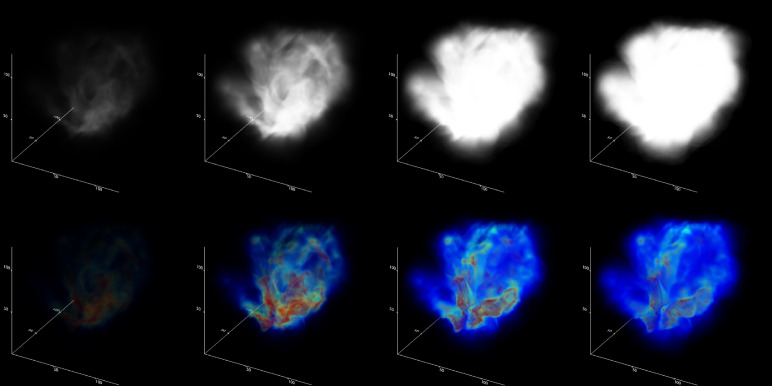
\includegraphics[width=1\linewidth]{figures/volume.jpg}
    \caption{An astronomy dataset visualisation generated by Frelled~\cite{Taylor2015} depicting how the addition of colour and opacity applied to the voxels effectively exposes hidden structures within the dataset. It shows how various ranges of opacity affect the visualisation but also how colour adds to its readability.}
    \label{fig:volume}
\end{figure*}

% Visualisation plays an integral role in allowing the visualisation to be interactively steered,
% the importance of visualisation and interaction for visual analysis is discussed further in Section \ref{visual-analytics}.

% visualisation challenges
There are certain characteristics present in the data which make visualisation difficult~\cite{Hassan2011}.
The datasets produced by astronomy data gathering instruments produce massive amounts of data, giga-bytes to peta-bytes, large enough to fill the memory of multiple conventional desktop computers.
This makes the datasets difficult to manage and process for visualisation.
There is no dominant file type used to represent astronomy data, which makes the development of a generic visualisation tool difficult.
Conventionally FITS files~\cite{wells1979} have been used to represent data cubes.
The cubes are divided up into slices along the \textit{z}-axis. 
Each of the these slices can be visualised as an image consisting of pixels with an \textit{x} and \textit{y} coordinate.
A user can move through slices of a data cube sequentially and can be played through like frames in a movie.
A major downside of visualising the data in this manner is that it does not let the user get an impression of how the dataset looks as a whole.
Therefore, limiting how quickly and effectively a user can construct a mental model and begin extracting insight~\cite{Norris1994}.
% bottleneck between human and machine where it is difficult for the user to construct model of the information in their mind in a way in which knowledge can be extracted
That data also has a high dynamic range and a low signal-to-noise ratio, which makes distinguishing genuine sources between large portions of noise difficult for astronomers.

\subsubsection{Visualisation Techniques}
There are different visualisation techniques which can be used to produce a representation of the dataset.
However, the nature of the data dictates the appropriate visualisation method to be used~\cite{Hassan2011}.
The common techniques used for generating comprehensive visualisations of a volume dataset are points, splats, iso-surfaces, and volume rendering.
% In the absence of a comprehensive visualisation, astronomers rely on techniques such as data-slicing or projected moment maps to aid research.
%\cite{Norris1994}% the most common techniques for representing astronomy volume data

\begin{figure}[h]
    \centering
    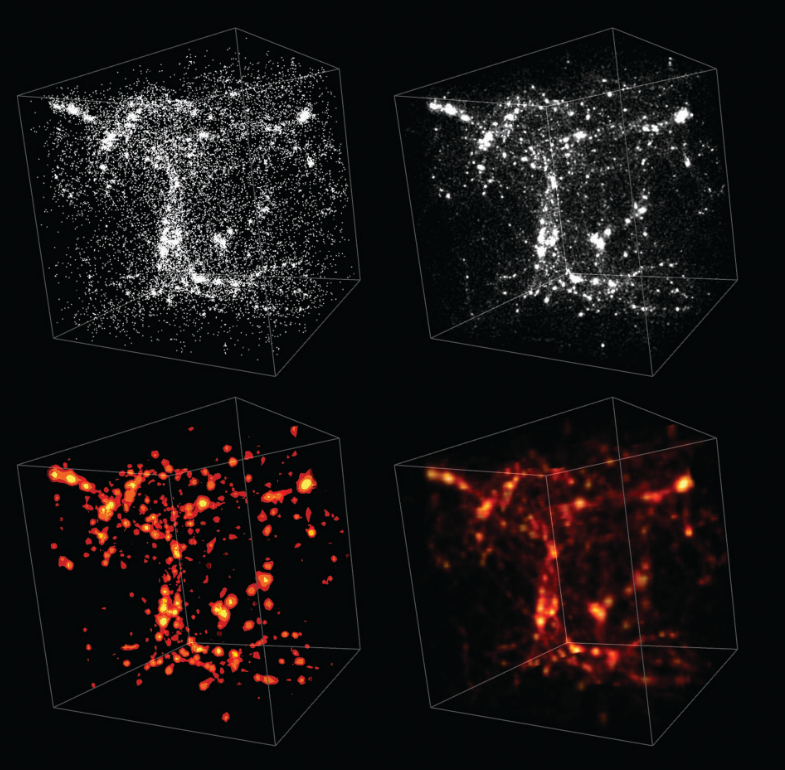
\includegraphics[width=\linewidth]{figures/visualisation.png}
    \caption{Four visualisations of an astronomy dataset using the common visualisation techniques~\cite{Hassan2011}, clearly depicting how the different visualisation techniques affect the presentation of the data. Point (top-left), splats (top-right), iso-surface (bottom-left), and volume rendering (bottom-right).}
    \label{fig:visualisation}
\end{figure}

\paragraph{Points}
% points
%   approach is limited by the available resolution (or pixeldensity) of the display
Each point in a dataset represented as a fixed-width pixel to a picture plane as if it were a three-dimensional scatter-plot.
While it is the most straightforward technique for representing data, this approach is limited by the available resolution or pixel density of a display.
This is not a suitable method for visualising astronomical data.
Simply plotting the data as a three-dimensional scatter plot makes it difficult to derive meaning from the data visualisation.
For example, the top left quadrant of Figure \ref{fig:visualisation} when compared to the bottom right quadrant is much less semantically comprehensible.

\paragraph{Splats}
This visualisation technique uses small two-dimensional textures to represent data points, and uses a method known as ``bill-boarding"~\cite{Taylor2015}, to ensure the textures always point towards the camera regardless of the scene's orientation.
When many splats are combined, this produces an effect that is much like volume rendering, but without the computational overhead of ray-tracing.

\paragraph{Iso-surface}
Polygon-based rendering, also referred to as surface rendering, is used to visualise volume data using polygons.
% three-dimensional equivalent of contouring
The majority of three-dimensional models use this method to represent their forms.
Surfaces or polygons must be extracted from volume data before it can be visualised.
Part of the visualisation process involves determining where the boundaries of the objects are and defining a skin for each region.
There are various methods for calculating these boundaries, such as: marching cubes, marching tetrahedra, multi-resolution iso-surface extraction, and surface wave propagation.
%   methods for calculating an isosurface from a data-set (check source for citations of the different methods)
Iso-surface rendering is commonly used to search for correlations between different scalar values, but is not used as a visualisation method because the visualisation is not comprehensive enough for knowledge extraction.
%   usually used to to searcg for correlation between different scalar values but are not as good at giving the overall picture of the dataset
% transparency is difficult
% boundaries could leave out interesting structures

\paragraph{Volume Rendering}
This technique renders each data point as three-dimensional pixels, also referred to as voxels. 
Voxels are arranged on the x-, y- and, z-axes to construct a three-dimensional image.
To make these structures more comprehensible, a colour transfer function is used to assign an opacity and colour to each voxel.
% volume rendering
%   provides a global view of the data-set
%   renders the external surfaces as well as the internal three-dimensional structure
%   ability to display weak or fuzzy surfaces
%   uses colour transfer function to assign an opacity and colour to the voxels
% uses ray-tracing or ray-marching shaders which can be computationally expensive
Volume rendering uses ray-tracing or ray-marching shaders to render the visualisation.
These types of shaders use significantly more computing resources compared to the traditional shading model~\cite{Wittenbrink2000}.
There are several optimisations and acceleration techniques that can tailor the shader to data being visualised.
% various algorithms for volume rendering
% back-to-front
% front-to-back
% shearing
% ray-casting
%   casts a ray from each pixel on the screen into the volume data along the viewing vector until it accumulates an opaque value
% ray-tracing
%   ray tracing is referred to as the process where reflected and transmitted rays are traced
However, it is a favoured method for representing volume data as it produces a complete view of the external surface as well as the internal three-dimensional structures within the dataset.

\subsubsection{Two-dimensional versus Three-dimensional Visualisations}
Three-dimensional visualisation techniques are better-suited for representing volume datasets, compared to two-dimensional visualisation techniques.
% why 3D is better suited for astronomy data than 2D visualisations

Some intuitive understanding of the data is missed when the data is examined using two-dimensional approaches~\cite{Kent2013}.
These approaches examine pieces of the data, such as individual slices from the dataset, or are played through sequentially like a movie.
This method of examination does not allow the user to observe the dataset as a whole.
% an intuitive understanding is missing when only examining data visualised with 2D approaches
% approaches where the iundividual channels or slices of a data cube are examined seperately 
Three-dimensional visualisations highlight hidden features within the data that would otherwise have remained hidden~\cite{Ferrand2016}.
% 3D vis techniques highight hidden features within the data that would have otherwise gone unnoticed
Comprehensive visualisations are important for communicating results quantitatively.
Therefore, visualisation which represent the data in a more comprehensive way is preferred.
% visualisation is important for communicating results quantitavely

%%%%%%%%%%%%%%%%%%%%%%%%%%%%%%%%%%%%%%%%%%%%%%%%%%%%

% challenges for petascale astronomy era
% \cite{Hassan2011}
% support of quantitative visualisation
% effective handling of large data-sets
% discovery in low signal-to-noise data
% better human-computer interaction and ubiquitous computing
% better workflow integrtion
% encouragement of adoption of 3D scientific visualisation techniques

%\cite{Hassan2011} % allow analysis to see the underlying large-scale structures hidden in the volumetric data set 
% by colour coding the points or applying a surface function to the data

% \cite{Sneiderman1996}
% mantra: overview first, zoom and filter, then details on demand
% seven data types (one-, two-, three-dimensional data, temporal and multi-dimensional data, and tree and network data)
% seven tasks (overview, Zoom, filter, details-on-demand, relate, history, and extracts).
% Exploring information collections becomes
% increasingly difficult as the volume grows.
% but the opportunity for dynamic displays takes user interface designers well beyond current wisdom. -> VR section in visual analytics
% Overall, the bandwidth of information presentation is potentially higher in the visual domain than for media reaching any of the other senses -> visual analytics section
% Users can scan, recognize, and recall images rapidly, and can detect changes in size, color, shape, movement, or texture

% \cite{Shneiderman2008}
% the purpose of visualising is insight not pictures
% the heart of information visualization is the well-designed user control panel and interaction techniques that enable users to generate task-related comprehensible coordinated windows
% The successful tools support a process of information-seeking that leads to important insights
% The successful visualization tools apply carefully designed data structures that run in the high speed store (RAM), so that even users of laptops with a few gigabytes of RAM can interactively explore million record databases.
% millions of records can translate to millions of data points within a volumetric dataset
% Billion record databases will require compression strategies or innovative hierarchical data management
% Precomputing of anticipated data needs can dramatically improve the user experience.

% \cite{Kaufman1996}
%  Volume visualization is a method of extracting information from volumetric datasets through interactive graphics and imaging, and is concerned with the representation, manipulation, and rendering of these datasets
% Volume data are 3D entities that may have information inside them, may not consist of surfaces and edges, or may be too voluminous to be represented geometrically.
% The primary sources of volume data are three: sampled data of real objects or phenomena, computed data produced by a computer simulation, and modeled data generated from a geometric model
% Examples of applications generating sampled data are medical imaging (e.g., CT, MRI), biology (e.g., confocal microscopy), geoscience (e.g., seismic measurements), industry (e.g., nondestructive inspection), and chemistry (e.g., electron density maps)
% volume cell (voxel for short), with each voxel being a rectangular cuboid havingsix faces, twelve edges, and eight corners.

% \cite{Kaufman1993}
% volume visualisation is a method for extracting meaningful information from volumetric datasets through the use of inteactive graphics and imaging. \cite{Rosenblum1994}
% provide mechanisims for peering inside volumetric datasets
% 3D voxel is the counterpart to the 2D pixel

% \cite{Rosenblum1994}
% that is, the basic ide a of using c omputer-generated pictures to gain information and understanding from data (geometry) and relationships (topology)

